%\ihead{\headmark}
\chapter{Deep Learning}

Deep learning is a subfield of machine learning which in fact, is a subfield of Artificial Intelligence (AI). Deep learning has emerged as one of the most exciting field of computer science, and it is keep expanding its scope. It has been used in many technologies such as, in medical to identify the diseases, automatic game playing, self-driving cars, image recognition, language translation and many more. The reason why deep learning is successful in many different domain is its ability to understand multiple levels of representation of data. Its mean that, it not only has ability to classify and predict, but also has ability to learn different level of complexity. Before diving into deep learning, it is necessary to understand a broader field "machine learning".

\subsection{Machine Learning}

Machine Learning [1] is a data analysis method. It gives the computer the ability to learn from data without being explicitly instructed. By using different machine learning algorithms, it helps to find hidden insights of data and allow us to build models to make predictions. It can be classified into 2 categories.

\begin{enumerate}
	\item Supervised Learning
	\item Unsupervised Learning
\end{enumerate}

\subsubsection{Supervised Learning}

In supervised learning, the labeled data is used to train the models. Here, labeled data represents that we know the input and output variables in advance. Thus, we know what we are looking for and then we use an algorithm to come up with a mapping function which maps the input variables to the output variables. Learning is supposed to be stopped when the level of performance reaches to the desired result. Supervised learning is generally divided into regression and classification.
\begin{itemize}
	\item \textbf{Regression}: A problem in which the output variable is a category.
	\item \textbf{Classification}: A problem in which the output variable is the real value.
\end{itemize}

\subsubsection{Unsupervised Learning}

In unsupervised learning, we only have input data and no corresponding output variables. Thus, there are no labels given and it is expected to find the structure in the data itself, i.e. finding hidden patterns to learn more about data. It is different from supervised learning in that we don't know what will be the correct value. Unsupervised learning is generally divided into clustering and association.

\begin{itemize}
	\item \textbf{Clustering}: Group objects in such a way that the objects, which are similar to each other, placed in the same cluster.
	\item \textbf{Association}: Discover rules that define the large portions of the data such as people who buys product X may buy Y as well.
\end{itemize}

The objective of machine learning is to analyze the past and present data and predict or make a decision for the future data. In supervised learning, the basic work flow is to build a model, evaluate or tune a model and then deploy it in the production environment where it will do the predictions. The work flow can be seen in figure.


\begin{figure}[htpb]
	\centering
	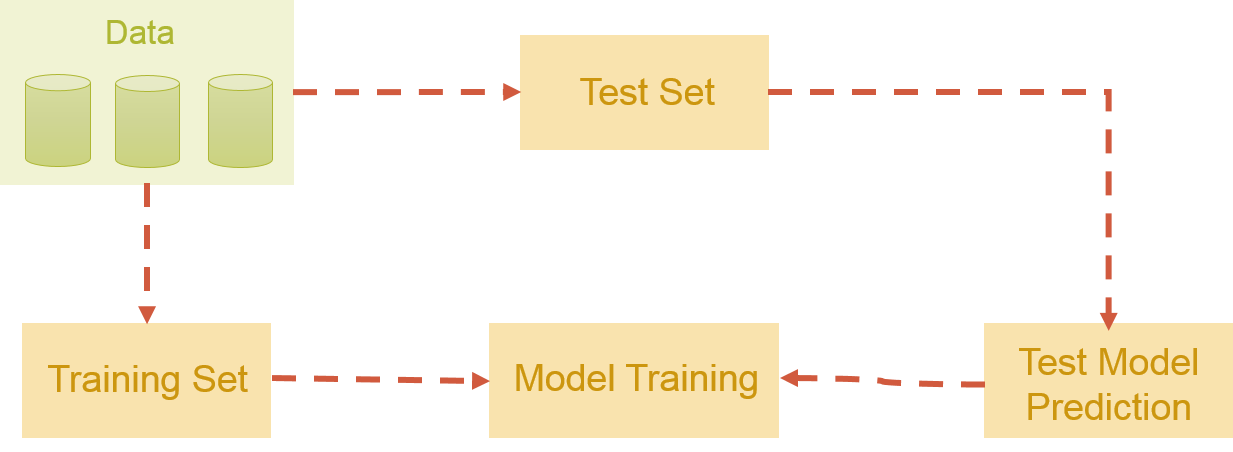
\includegraphics[width=12cm,height=10cm,keepaspectratio=true]{images/basic-ml-model.png}
	\caption{
		Basic supervised machine learning workflow.
	}
	\label{fig:basic-ml-model}
\end{figure}


One of the problem with the traditional machine learning model is the feature extraction challenge. The model designer or the programmer needs to specifically tells the model which features it should consider to make a correct decision. The model heavily relies on the programmer's understanding of data and this was a huge burden on the programmers. For a problems like object recognition, language translation, it was a huge problem.

Deep learning comes into play to solve the problem of feature extraction. They have the capability to focus only on the right features by themselves by understanding as much data as possible, requiring very little input from the programmer. This feature of deep learning models makes it very powerful tool for the current machine learning era.

\section{Artificial Neural Networks}


